\documentclass[spanish,a4paper]{article}

% Paquetes generales
\usepackage{ifthen}
\usepackage{amssymb}
\usepackage{amsmath}
\usepackage{multicol}
\usepackage[absolute]{textpos}
\usepackage{hyperref}

% Cuestiones de enunciados

% Primero definiciones de cosas al estilo title, author, date
\def\materia#1{\gdef\@materia{#1}}
\def\@materia{M\'{e}todos Num\'{e}ricos}
\def\lamateria{\@materia}

\def\cuatrimestre#1{\gdef\@cuatrimestre{#1}}
\def\@cuatrimestre{No especifi\'o el cuatrimestre}
\def\elcuatrimestre{\@cuatrimestre}

\def\anio#1{\gdef\@anio{#1}}
\def\@anio{No especifi\'o el anio}
\def\elanio{\@anio}

\def\fecha#1{\gdef\@fecha{#1}}
\def\@fecha{\today}
\def\lafecha{\@fecha}

\def\nombre#1{\gdef\@nombre{#1}}
\def\@nombre{No especific'o el nombre}
\def\elnombre{\@nombre}

\def\practica#1{\gdef\@practica{#1}}
\def\@practica{No especifi\'o el n\'umero de pr\'actica}
\def\lapractica{\@practica}

% Esta macro convierte el numero de cuatrimestre a palabras
\newcommand{\cuatrimestreLindo}{
  \ifthenelse{\equal{\elcuatrimestre}{1}}
  {Primer cuatrimestre}
  {\ifthenelse{\equal{\elcuatrimestre}{2}}
  {Segundo cuatrimestre}
  {Verano}}
}

\newcommand{\depto}{{UBA -- Facultad de Ciencias Exactas y Naturales --
      Departamento de Computaci\'on}}

\newcommand{\titulopractica}{
  \centerline{\depto}
  \vspace{1ex}
  \centerline{{\Large\lamateria}}
  \vspace{0.5ex}
  \centerline{\cuatrimestreLindo de \elanio}
  \vspace{2ex}
  \centerline{{\huge Pr\'actica \lapractica -- \elnombre}}
  \vspace{5ex}
  \arreglarincisos
  \newcounter{ejercicio}
  \newenvironment{ejercicio}{\stepcounter{ejercicio}\textbf{Ejercicio
      \theejercicio}%
    \renewcommand\@currentlabel{\theejercicio}%
  }{\vspace{0.2cm}}
}  

\newcommand{\titulotp}{
  \centerline{\depto}
  \vspace{1ex}
  \centerline{{\Large\lamateria}}
  \vspace{0.5ex}
  \centerline{\cuatrimestreLindo de \elanio}
  \vspace{0.5ex}
  \centerline{\lafecha}
  \vspace{2ex}
  \centerline{{\huge\elnombre}}
  \vspace{5ex}
}

\usepackage[spanish]{babel}
\selectlanguage{spanish}
\usepackage[utf8]{inputenc}
%\usepackage{bbm}
\usepackage{framed}


\newcommand{\comen}[2]{%
\begin{framed}
\noindent \textsf{#1:} #2
\end{framed}
}

% **************************************************************************
%
%  Package 'caratula', version 0.5 (para componer caratulas de TPs del DC).
%
%  En caso de dudas, problemas o sugerencias sobre este package escribir a
%  Brian J. Cardiff (bcardif arroba gmail.com).
%  Nico Rosner (nrosner arroba dc.uba.ar).
%
% **************************************************************************

% ----- Informacion sobre el package para el sistema -----------------------

\NeedsTeXFormat{LaTeX2e}
\ProvidesPackage{caratula}[2013/08/04 v0.5 Para componer caratulas de TPs del DC]
\RequirePackage{ifthen}
\usepackage[pdftex]{graphicx}

% ----- Imprimir un mensajito al procesar un .tex que use este package -----

\typeout{Cargando package 'caratula' v0.5 (2013/08/04)}

% ----- Algunas variables --------------------------------------------------

\let\Materia\relax
\let\Submateria\relax
\let\Titulo\relax
\let\Subtitulo\relax
\let\Grupo\relax
\let\Fecha\relax
\let\Logoimagefile\relax
\newcommand{\LabelIntegrantes}{}
\newboolean{showLU}
\newboolean{showEntregas}
\newboolean{showDirectores}

% ----- Comandos para que el usuario defina las variables ------------------

\def\materia#1{\def\Materia{#1}}
\def\submateria#1{\def\Submateria{#1}}
\def\titulo#1{\def\Titulo{#1}}
\def\subtitulo#1{\def\Subtitulo{#1}}
\def\grupo#1{\def\Grupo{#1}}
\def\fecha#1{\def\Fecha{#1}}
\def\logoimagefile#1{\def\Logoimagefile{#1}}

% ----- Token list para los integrantes ------------------------------------

\newtoks\intlist\intlist={}

\newtoks\intlistSinLU\intlistSinLU={}

\newcounter{integrantesCount}
\setcounter{integrantesCount}{0}
\newtoks\intTabNombre\intTabNombre={}
\newtoks\intTabLU\intTabLU={}
\newtoks\intTabEmail\intTabEmail={}

\newcounter{directoresCount}
\setcounter{directoresCount}{0}
\newtoks\direcTabNombre\direcTabNombre={}
\newtoks\direcTabEmail\direcTabEmail={}

% ----- Comando para que el usuario agregue integrantes --------------------

\def\integrante#1#2#3{%
    \intlist=\expandafter{\the\intlist\rule{0pt}{1.2em}#1&#2&\tt #3\\[0.2em]}%
    \intlistSinLU=\expandafter{\the\intlistSinLU\rule{0pt}{1.2em}#1 & \tt #3\\[0.2em]}%
    %
    \ifthenelse{\value{integrantesCount} > 0}{%
        \intTabNombre=\expandafter{\the\intTabNombre & #1}%
        \intTabLU=\expandafter{\the\intTabLU & #2}%
        \intTabEmail=\expandafter{\the\intTabEmail & \tt #3}%
    }{
        \intTabNombre=\expandafter{\the\intTabNombre #1}%
        \intTabLU=\expandafter{\the\intTabLU #2}%
        \intTabEmail=\expandafter{\the\intTabEmail \tt #3}%
    }%
    \addtocounter{integrantesCount}{1}%
}

\def\director#1#2{%
    \ifthenelse{\value{directoresCount} > 0}{%
        \direcTabNombre=\expandafter{\the\direcTabNombre & #1}%
        \direcTabEmail=\expandafter{\the\direcTabEmail & \tt #2}%
    }{
        \direcTabNombre=\expandafter{\the\direcTabNombre #1}%
        \direcTabEmail=\expandafter{\the\direcTabEmail \tt #2}%
    }%
    \addtocounter{directoresCount}{1}%
}

% ----- Macro para generar la tabla de integrantes -------------------------

\newcommand{\tablaIntegrantes}{\ }

\newcommand{\tablaIntegrantesVertical}{%
\ifthenelse{\boolean{showLU}}{%
    \begin{tabular}[t]{| l @{\hspace{4ex}} c @{\hspace{4ex}} l|}
        \hline
        \multicolumn{1}{|c}{\rule{0pt}{1.2em} \LabelIntegrantes} & LU &  \multicolumn{1}{c|}{Correo electr\'onico} \\[0.2em]
        \hline \hline
        \the\intlist
        \hline
    \end{tabular}
}{
    \begin{tabular}[t]{| l @{\hspace{4ex}} @{\hspace{4ex}} l|}
        \hline
        \multicolumn{1}{|c}{\rule{0pt}{1.2em} \LabelIntegrantes} &  \multicolumn{1}{c|}{Correo electr\'onico} \\[0.2em]
        \hline \hline
        \the\intlistSinLU
        \hline
    \end{tabular}
    }%
}

\newcommand{\tablaIntegrantesHorizontal}{%
    \begin{tabular}[t]{ *{\value{integrantesCount}}{c} }
    \the\intTabNombre \\%
\ifthenelse{\boolean{showLU}}{
    \the\intTabLU \\%
}{}
    \the\intTabEmail %
    \end{tabular}%
}

\newcommand{\tablaDirectores}{%
\ifthenelse{\boolean{showDirectores}}{%
    \bigskip
    Directores

    \smallskip
    \begin{tabular}[t]{ *{\value{directoresCount}}{c} }
    \the\direcTabNombre \\%
    \the\direcTabEmail %
    \end{tabular}%
}{}%
}

\newcommand{\tablaEntregas}{%
\ifthenelse{\boolean{showEntregas}}{%
  \bigskip%
  \begin{tabular}[t]{|l p{3.5cm} p{1.5cm}|}%
  \hline%
  \rule{0pt}{1.2em} Instancia & Docente & Nota \\[0.2em] %
  \hline%
  \hline%
  \rule{0pt}{1.2em} Primera entrega & & \\[0.2em] %
  \hline%
  \rule{0pt}{1.2em} Segunda entrega & & \\[0.2em] %
  \hline%
  \end{tabular}%
}{}%
}

% ----- Codigo para manejo de errores --------------------------------------

\def\se{\let\ifsetuperror\iftrue}
\def\ifsetuperror{%
    \let\ifsetuperror\iffalse
    \ifx\Materia\relax\se\errhelp={Te olvidaste de proveer una \materia{}.}\fi
    \ifx\Titulo\relax\se\errhelp={Te olvidaste de proveer un \titulo{}.}\fi
    \edef\mlist{\the\intlist}\ifx\mlist\empty\se%
    \errhelp={Tenes que proveer al menos un \integrante{nombre}{lu}{email}.}\fi
    \expandafter\ifsetuperror}

\def\aftermaketitle{%
  \setcounter{page}{1}
}

% ----- \maketitletxt correspondiente a la versi�n v0.2.1 (texto v0.2 + fecha ) ---------

\def\maketitletxt{%
    \ifsetuperror\errmessage{Faltan datos de la caratula! Ingresar 'h' para mas informacion.}\fi
    \thispagestyle{empty}
    \begin{center}
    \vspace*{\stretch{2}}
    {\LARGE\textbf{\Materia}}\\[1em]
    \ifx\Submateria\relax\else{\Large \Submateria}\\[0.5em]\fi
    \ifx\Fecha\relax\else{\Large \Fecha}\\[0.5em]\fi
    \par\vspace{\stretch{1}}
    {\large Departamento de Computaci\'on}\\[0.5em]
    {\large Facultad de Ciencias Exactas y Naturales}\\[0.5em]
    {\large Universidad de Buenos Aires}
    \par\vspace{\stretch{3}}
    {\Large \textbf{\Titulo}}\\[0.8em]
    {\Large \Subtitulo}
    \par\vspace{\stretch{3}}
    \ifx\Grupo\relax\else\textbf{\Grupo}\par\bigskip\fi
    \tablaIntegrantes
    \end{center}
    \vspace*{\stretch{3}}
    \newpage\aftermaketitle}

% ----- \maketitletxtlogo correspondiente v0.2.1 (texto con fecha y logo) ---------

\def\maketitletxtlogo{%
    \ifsetuperror\errmessage{Faltan datos de la caratula! Ingresar 'h' para mas informacion.}\fi
    \thispagestyle{empty}
    \begin{center}
    \ifx\Logoimagefile\relax\else\includegraphics{\Logoimagefile}\fi \hfill 
\includegraphics{logo_dc.jpg}\\[1em]
    \vspace*{\stretch{2}}
    {\LARGE\textbf{\Materia}}\\[1em]
    \ifx\Submateria\relax\else{\Large \Submateria}\\[0.5em]\fi
    \ifx\Fecha\relax\else{\large \Fecha}\\[0.5em]\fi
    \par\vspace{\stretch{1}}
    {\large Departamento de Computaci\'on}\\[0.5em]
    {\large Facultad de Ciencias Exactas y Naturales}\\[0.5em]
    {\large Universidad de Buenos Aires}
    \par\vspace{\stretch{3}}
    {\Large \textbf{\Titulo}}\\[0.8em]
    {\Large \Subtitulo}
    \par\vspace{\stretch{3}}
    \ifx\Grupo\relax\else\textbf{\Grupo}\par\bigskip\fi
    \tablaIntegrantes
    \end{center}
    \vspace*{\stretch{4}}
    \newpage\aftermaketitle}

% ----- \maketitlegraf correspondiente a la versi�n v0.3 (gr�fica) -------------

\def\maketitlegraf{%
    \ifsetuperror\errmessage{Faltan datos de la caratula! Ingresar 'h' para mas informacion.}\fi
%
    \thispagestyle{empty}

    \ifx\Logoimagefile\relax\else\includegraphics{\Logoimagefile}\fi \hfill 
\includegraphics{logo_dc.jpg}

    \vspace*{.06 \textheight}

    \noindent \textbf{\huge \Titulo}  \medskip \\
    \ifx\Subtitulo\relax\else\noindent\textbf{\large \Subtitulo} \\ \fi%
    \noindent \rule{\textwidth}{1 pt}

    {\noindent\large\Fecha \hspace*\fill \Materia} \\
    \ifx\Submateria\relax\else{\noindent \hspace*\fill \Submateria}\fi%

    \medskip%
    \begin{center}
        \ifx\Grupo\relax\else\textbf{\Grupo}\par\bigskip\fi
        \tablaIntegrantes

        \tablaDirectores

        \tablaEntregas
    \end{center}%
    \vfill%
%
    \begin{minipage}[t]{\textwidth}
        \begin{minipage}[t]{.55 \textwidth}
            
\includegraphics{logo_uba.jpg}
        \end{minipage}%%
        \begin{minipage}[b]{.45 \textwidth}
            \textbf{\textsf{Facultad de Ciencias Exactas y Naturales}} \\
            \textsf{Universidad de Buenos Aires} \\
            {\scriptsize %
            Ciudad Universitaria - (Pabell\'on I/Planta Baja) \\
                Intendente G\"uiraldes 2160 - C1428EGA \\
            Ciudad Aut\'onoma de Buenos Aires - Rep. Argentina \\
                Tel/Fax: (54 11) 4576-3359 \\
            http://www.fcen.uba.ar \\
            }
        \end{minipage}
    \end{minipage}%
%
    \newpage\aftermaketitle}

% ----- Reemplazamos el comando \maketitle de LaTeX con el nuestro ---------
\renewcommand{\maketitle}{\maketitlegraf}

% ----- Dependiendo de las opciones ---------
%
% opciones:
%   txt     : caratula solo texto.
%   txtlogo : caratula txt con logo del DC y del grupo (opcional).
%   graf    : (default) caratula grafica con logo del DC, UBA y del grupo (opcional).
%
%\@makeother\*% some package redefined it as a letter (as color.sty)
%
% Layout general de la caratula
%
\DeclareOption{txt}{\renewcommand{\maketitle}{\maketitletxt}}
\DeclareOption{txtlogo}{\renewcommand{\maketitle}{\maketitletxtlogo}}
\DeclareOption{graf}{\renewcommand{\maketitle}{\maketitlegraf}}
%
% Etiqueta Autores o Integrantes
%
\DeclareOption{integrante}{\renewcommand{\LabelIntegrantes}{Integrante}}
\DeclareOption{autor}{\renewcommand{\LabelIntegrantes}{Autor}}
%
% Formato tabla de integrantes
%
\DeclareOption{intVert}{\renewcommand{\tablaIntegrantes}{\tablaIntegrantesVertical}}
\DeclareOption{intHoriz}{\renewcommand{\tablaIntegrantes}{\tablaIntegrantesHorizontal}}
\DeclareOption{conLU}{\setboolean{showLU}{true}}
\DeclareOption{sinLU}{\setboolean{showLU}{false}}
\DeclareOption{conEntregas}{\setboolean{showEntregas}{true}}
\DeclareOption{sinEntregas}{\setboolean{showEntregas}{false}}
\DeclareOption{showDirectores}{\setboolean{showDirectores}{true}}
\DeclareOption{hideDirectores}{\setboolean{showDirectores}{false}}
%
% Opciones predeterminadas
%
\ExecuteOptions{intVert}%
\ExecuteOptions{graf}%
\ExecuteOptions{integrante}%
\ExecuteOptions{conLU}%
\ExecuteOptions{hideDirectores}%
\ExecuteOptions{sinEntregas}%
%
\ProcessOptions\relax

\begin{document}

\materia{}

\titulo{M\'{e}todos Num\'{e}ricos}
\subtitulo{TP 1: "No creo que a  \'{e}l le gustara eso"}

\fecha{\today}


\grupo{}

\integrante{Fosco, Martin Esteban}{449/13}{mfosco2005@yahoo.com.ar}
\integrante{Minces Müller, Javier Nicolás}{231/13}{javijavi1994@gmail.com}
\integrante{Chibana, Christian Tomokazu De La Vega Jr.}{}{tomistomus@LaMilagrosa.com.jp}



\maketitle

\clearpage

\nombre{\LARGE }

\LARGE \textbf{Resumen}
\normalsize

En este trabajo implementamos una solución al problema planteado en el tp, encontrar una manera de determinar qué sanguijuelas pegadas al parabrisas son peligrosas y eliminarlas, usando una representación matricial del sistema de ecuaciones que nos permita hallar la temperatura del parabrisas en cada punto (con una precisión determinada por la granularidad) tomando como incógnitas a, justamente, cada punto del parabrisas.\newline
Para resolver dicho sistema de ecuaciones recurrimos a técnicas matemáticas basadas en métodos de resolución de sistemas, y dividimos en distintos módulos (structs) con funciones específicas al parabrisas y a la matriz del sistema de ecuaciones para facilitar la comprensión (tanto de los docentes como de nosotros mismos) de la implementación hecha.%para facilitar la comprensión? en serio?

\newpage

\LARGE \textbf{Índice}
\normalsize

\flushleft

\ref{sec:intro}{              Introducción Teórica}\newline \newline 
\ref{sec:desarrollo}{              Desarrollo}\newline \newline
\ref{sec:res}{              Resultados}\newline \newline
\ref{sec:discusion}{              Discusión}\newline \newline
\ref{sec:conclusiones}{              Conclusiones}\newline \newline
\ref{sec:ApA}{              Apéndice A}\newline \newline
\ref{sec:ref}{              Referencias}


\newpage

\section{Introducci\'{o}n Te\'{o}rica}
\label{sec:intro}

El objetivo de este trabajo es usar métodos numéricos para la resolución de sistemas de ecuaciones, observándolos como una matriz multiplicada por un vector incógnita, de este producto obtenemos un vector resultado (este vector resultado representa el valor en cada punto

Para resolver nuestro sistema de ecuaciones (expresado en forma de una matriz) se usó el método conocido como "Eliminación Gaussiana", que nos permite triangular una matriz de forma relativamente eficiente (es decir llegar de una matriz común a una triangular superior) recurriendo a la resta e intercambio entre filas de la misma matriz (con un multiplicador que sirva para reducir los valores por debajo de la diagonal a 0). 

Como dato, se tenía que cada punto del parabrisas satisfacía la ecuación de Laplace.\newline $\frac{\partial ^2u}{\partial x^2}+\frac{\partial ^2u}{\partial y^2}=0$

Aplicando el modelo de aproximación por diferencias finitas se puede ver que la temperatura de cada punto desconocido puede expresarse como el promedio de cada uno de los puntos adyacentes. Es decir, la temperatura de cada punto del parabrisas se puede expresar como una ecuación lineal:  \newline 

$\left \{\begin{matrix}
\frac{1}{4}x_{i+1,j}+\frac{1}{4}x_{i,j+1}+\frac{1}{4}x_{i-1,j}+\frac{1}{4}x_{i,j-1}-x_{i,j}=0 \text{ si el punto es desconocido} \\  x_{i,j}=-100 \text{ si el punto es borde} \\ x_{i,j}=temp \text{ si el punto es sanguijuela} \end{matrix}$

Considerando todos los puntos desconocidos de la matriz, se obtuvo entonces un sistema de ecuaciones lineales de a+l x a+l, siendo a y l el ancho y el largo de la matriz parabrisas, respectivamente.

\newpage

\section{Desarrollo}
\label{sec:desarrollo}

Nuestro trabajo apunta a resolver un problema que afrontamos dividiéndolo en tres partes. \newline \newline
La \textbf{Primera parte} del problema consistía en hallar una forma de representar el calor causado por unas sanguijuelas en un parabrisas rectangular en un momento determinado (este momento no esta especificado, sólo recibimos los datos relevantes correspondientes a dicho momento como argumento) representando dicho parabrisas como una matriz y utilizando el lenguaje C++. Algunos puntos son conocidos, ya que el parabrisas tiene bordes con una temperatura constante, y fuentes de calor (sanguijuelas) con radio y temperatura a determinar por los parámetros r y t.

Para poder modelar el parabrisas se tomó una discretización, con granularidad variable. De esta forma, el parabrisas quedó representado con una matriz de a/h+1 filas y l/h+1 columnas, siendo a el ancho en metros del parabrisas original, l su largo y h la granularidad elegida y l su largo. A esta matriz la llamaremos "matriz parabrisas".

%sé que acá va lo de intentos fallidos y esas cosas, y eso que dijo el tipo que pongamos en algún lado de por qué no guardamos solo el vector de 1s y -1s
Nuestro problema entonces se reducía a plantear una resolución:
En un principio pensamos en utilizar una sola estructura para el problema, una matriz que generara la matriz a partir de los datos leídos en el archivo de entrada (que nos indica los datos relevantes para hallar la temperatura en cada punto del parabrisas). El problema que encontramos era que al crear la matriz, solo guardábamos sus celdas, perdiendo los datos originales del problema. De esta forma, no podíamos generar la matriz parabrisas sin el saber su ancho, para devolver los datos de la forma requerida. Guardar estos datos como parte de la estructura hubiera sido una solución forzada, que hubiera hecho que la matriz dejara de ser una estructura genérica para volverse específica de este problema. Por eso, optamos por una estructura parabrisas, que guardara todos los datos relevantes.

Por ejemplo, sea una matriz parabrisas de 3x3: \newline \newline

$\begin{bmatrix}x_{11}&x_{12}&x_{13}\\x_{21}&x_{22}&x_{23}\\x_{31}&x_{32}&x_{33}\end{bmatrix}$ \newline \newline

El sistema de ecuaciones queda planteado de esta forma: \newline \newline

$\begin{bmatrix}1&0&0&0&0&0&0&0&0\\0&1&0&0&0&0&0&0&0\\0&0&1&0&0&0&0&0&0\\0&0&0&1&0&0&0&0&0\\0&\frac{1}{4}&0&\frac{1}{4}&-1&\frac{1}{4}&0&\frac{1}{4}&0\\0&0&0&0&0&1&0&0&0\\0&0&0&0&0&0&1&0&0\\0&0&0&0&0&0&0&1&0\\0&0&0&0&0&0&0&0&1\end{bmatrix} \begin{bmatrix}x_{11}\\x_{12}\\x_{13}\\x_{21}\\x_{22}\\x_{23}\\x_{31}\\x_{32}\\x_{33}\end{bmatrix} \begin{bmatrix}-100\\-100\\-100\\-100\\0\\-100\\-100\\-100\\-100\end{bmatrix}$ \newline \newline

Para almacenar la matriz se usaron dos métodos. El primero fue un vector de filas, donde cada fila era un vector con todos sus valores. Para el segundo aprovechamos la estructura banda de la matriz (¿explicar/definir?/desarrollar) para almacenar, de cada fila, solo los elementos que forman parte de la banda. Al triangular, la matriz mantiene su ancho de banda.

Para aprovechar la estructura banda se pensó en guardar únicamente un vector de valores booleanos que permitiera saber para cada celda de la matriz parabrisas si su valor era conocido o desconocido, ya que solo con ese dato era posible saber el valor de toda la fila de la otra matriz. Sin embargo, esta estructura no puede mantenerse al triangular, ya que el valor de la fila toma valores que no dependen únicamente de la celda que representa. 

Finalmente, para implementar la matriz banda, no creamos otra estructura, sino que modificamos la estructura matriz ya existente, de forma que incluyera un booleano que dijera si era una matriz banda, y un entero que indicara el ancho de banda. De esta forma, todas las operaciones de la matriz podían utilizarse para la matriz banda, con la única exepción de la función que permite definir un valor en una celda y la que busca el valor de una celda determinada, en las que hubo que separar en dos casos.

Al implementar esto, hubo que modificar el algoritmo que crea la matriz a partir de un parabrisas para que solo definiera los elementos de la banda. También hubo que modificar indirectamente la eliminación gaussiana, ya que al restar filas solo debían tenerse en cuenta las celdas que formaran parte de la banda. El ancho de banda es 2 x a + 1, donde a es el ancho de la matriz parabrisas.

La \textbf{Segunda parte} se trataba de experimentar con estos algoritmos desarrollados y comparar tiempos y espacio ocupados por cada implementación, que resolvimos probando diferentes experimentos, y comparando el rendimiento de ambas implementaciones (la banda se desempeñó de forma más eficiente, pero más detalles sobre esto se darán en la sección de implementación)\newline \newline

La \textbf{Tercera parte} del problema consistía en encontrar un algoritmo que permitiera elegir qué sanguijuelas eliminar para que la temperatura del punto crítico del vidrio se mantuviera por debajo de 235º, evitando eliminar más sanguijuelas de las estrictamente necesarias. Nuestro algoritmo fue heurístico: elegimos que se eliminara siempre la sanguijuela más cercana al centro. Elegimos hacerlo de esta manera porque la sanguijuela que más influye en la temperatura de un punto es la más cercana, siendo el borde fijo.\newline
Una opción más provechosa en términos del uso de láseres sería usar un algoritmo que antes de decidir si eliminar una sanguijuela simulara el estado del punto crítico posterior a su eliminación, haciendo esta simulación con todas las sanguijuelas (o con todas dentro un determinado radio); luego podría elegir una sanguijuela a eliminar observando en cuál estado posterior de la simulación el punto crítico bajó más.
Un ejemplo de un caso en el que este último algoritmo se desempeña mejor sería si tomamos un caso en el que tenemos diez sanguijuelas muy cerca una de la otra y del punto crítico y una no tan cerca, pero en el que eliminar esta sanguijuela solitaria bastaría para reducir la temperatura del punto crítico a un valor óptimo.
El algoritmo que elegimos iría por la "fuerza bruta" y eliminaría las 10 sanguijuelas más cercanas.
El algoritmo más eficiente (en uso de lásers), en cambio, notaría que eliminando una sola sanguijuela puede alcanzar un resultado aceptable, y al ver que eliminando una sola de las sangujuelas más cercanas no conseguiría nada, elegiría entonces a la más lejana, matando una sola sanguijuela.

Sin embargo, nos inclinamos por el algoritmo de fuerza bruta debido a que consideramos que el costo del algoritmo más inteligente tanto en complejidad de programación, temporal y espacial sería mucho mayor, debido a que debería correr 11 veces la simulación para decidirse por una sanguijuela, mientras que el de fuerza bruta sólo una. Además, conisderamos altamente imporbable que se dé un ejemplo así.

Decidimos implementar el algoritmo de forma que imprimiera en un archivo separado una lista de las sanguijuelas eliminadsas, en orden, junto con la temperatura en el punto crítico después de cada eliminación. Dado que después de cada eliminación era necesario recalcular todo el sistema, usamos para esto el algoritmo de matriz banda. \newline \newline

%Inicialmente trabajamos con tolerancia, forzando un 0 cuando el valor de una celda era menor a $10^{-10}$ en módulo, 

\newpage

\section{Resultados}
\label{sec:res}

Tiempo de ejecución según la granularidad
Valores de entrada: (los busco después)
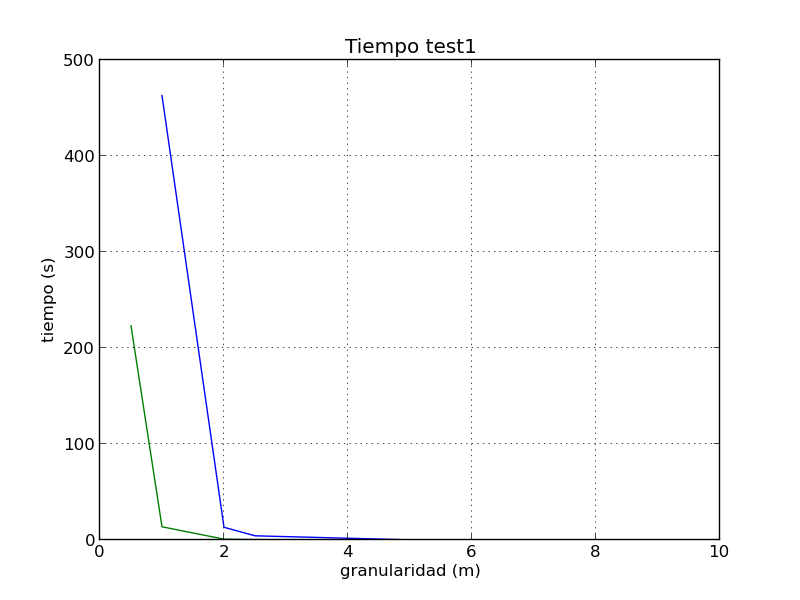
\includegraphics[width=250pt]{test.png}

%<<Copiar y pegar un LSD.out>>

%Y si les parece poco chamuyamos con lo de que cambiar la granularidad afecta la temperatura del punto medio

%Consigna:
%Considerar al menos dos instancias de prueba, generando discretizaciones variando la granularidad para cada una de ellas y comparando el valor de la temperatura en el punto
%crítico. Se sugiere presentar gráficos de temperatura para los mismos, ya sea utilizando las herramientas provistas por la cátedra o implementando sus propias herramientas de
%graficación.
%
%Analizar el tiempo de cómputo requerido en función de la granularidad de la discretización, buscando un compromiso entre la calidad de la solución obtenida y el tiempo de cómputo %requerido. Comparar los resultados obtenidos para las variantes propuestas en 1 y 2.

% Estudiar el comportamiento del método propuesto para la estimación de la temperatura
%en el punto crítico y para la eliminación de sanguijuelas.

\newpage

\section{Discusi\'{o}n}
\label{sec:discusion}

Para analizar los resultados tomaremos en cuenta el orden de complejidad asintótico O. Llamaremos l al largo de la matriz parabrisas, l' al largo del parabrisas, a al ancho de la matriz parabrisas, a' al ancho del parabrisas y h a la granularidad, 

Teniendo en cuenta que la matriz cuadrada es de (l x a) x (l x a) y que la matriz banda solo debe conservar (l x a) x (2 x a + 1) valores, la matriz banda ocupa menos memoria cuando l > 2. La diferencia escala con l. En el caso asintótico, ocupa $O(l^2\ a^2)$ la matriz cuadrada y $O(l a^2)$ la matriz banda. \endline \endline


En cuanto al costo temporal, podemos separar cada parte de la implementación:\endline \endline
 %Esto es más bien hipótesis, lo que haría que comparar es después esto con los resultados
\begin{tabular}{ l c r }
  Operación & Costo matriz común & Costo matriz banda \\
  Cargar los datos & O(k) [1] \\
  Generar la matriz & O($(al)^2$) & O($a^2l$)\\
  Triangular la matriz & O($(al)^3$) & O($a^3l^2$) \\
  Generar el vector de resultados & O($(al)^2$) & O($(al)^2$)\\
  Imprimir el vector de resultados & O($al$) & O($al$)\\
  Tiempo total de ejecución [1] & O($(al)^3$) & O($a^3l^2$)\endline\endline
\end{tabular} 

[1] Donde k es la cantidad de sanguijuelas 

[2] Si acotamos la cantidad de sanguijuelas por el tamaño de la matriz parabrisas \\ 


Se tiene que lo que determina el costo total es la tirangulación de la matriz. Por eso, el algoritmo banda es temporalmente más eficiente que el algoritmo de eliminación gaussiana común. Esto se debe a la operación que resta filas, que se ejecuta hasta $((al)^2)/2$ veces, siendo a y l ancho y largo de la matriz parabrisas, ya que puede ser necesario ejecutarla una vez para generar un 0 en cada celda por debajo de la diagonal. (ejemplos y tabla). %Ok, acá SI hay muchas comas
Esta operación tiene como complejidad al en el caso de la matriz comúm, y 2a+1 en el caso de la matriz banda, ya que solo debe restar las celdas que forman parte de la banda, cuya cantidad corresponde con el ancho de banda. La complejidad total de la triangulación es, entonces, O($(la)^3$) en el caso de la matriz común y O($l^2 a^3$) en el caso de la banda. Esto se puede ver en los gráficos de tiempo de ejecución. % o debería

Como se puede ver de los gráficos de tiempo de ejecución, al reducirse la granularidad, aumenta el tiempo de ejecución. Esto es porque reducir al doble la granularidad, por ejemplo, implica duplicar tanto el largo como el ancho de la matriz parabrisas. Si consideramos l=l'/h+1 y a=a'/h+1, podemos reescribir los órdens de complejidad de los algoritmos. El algoritmo de triangulación de la matriz común cuesta O($\frac{l'^3 a'^3}{h^6}$) y el de la matriz banda, O($\frac{l'^2 a'^3}{h^5}$). Entonces, por ejemplo reducir a la mitad la granularidad implica aumentar 64 veces el tiempo de ejecución en un caso y 32 en el otro. %unciona así?


Algo del algoritmo de eliminación. Por ejemplo, que al eliminar cada sanguijuela baja la temperatura, salvo que haya dos en exactamente el mismo lugar. Eso habla bien del algoritmo. Algo de cuánto tarda, por ejemplo, comparando con un algortimo que asegure ser óptimo.

\newpage

\section{Conclusiones}
\label{sec:conclusiones}

Todo esto ya lo puse en discusión:
%La banda es más rápida (¿cuanto?) y ocupa menos memoria (¿cuanto?) %(no, en serio?)
%Reducir n veces la granularidad implica aumentar el tiempo de ejecución n^6 veces en el caso de la matriz común y n^5 en el caso de la banda %(ponele, hay comparar con los resultados) <-Puede ser que esto vaya en discusión y en las conclusiones solo algo más general?

El tiempo de ejecución no depende de la cantidad de sanguijuelas, salvo porque puede implicar más puntos determinados.


Algo de factorización LU?
\newpage
\section{Apéndice A}
\label{sec:ApA}

%<<Copiar enunciado, lo haría yo pero se van a ilusionar con que de golpe tenemos 10 páginas>>
%y si quieren apéndice B: algoritmos en pseudocódigo \forall

\newpage

\section{Referencias}
\label{sec:ref}

%Roulinsson, Rouli, "Como hacer el TP de Métodos for dummies", Ed. edificio dorado, 2014

%Eh, no sé, yo en el secundario siempre puse apuntes de clase y si quieren pongan el libro que sea el de la materia, aunque si lo toco para el final va a ser como :O

\end{document}
